\documentclass[12pt, titlepage]{article}
\usepackage[french]{babel}
\usepackage[utf8]{inputenc}
\usepackage[T1]{fontenc}
\usepackage[a4paper, margin=0.7in]{geometry}
\usepackage[utf8]{inputenc}
\usepackage{graphicx}
\usepackage{hyperref}
\usepackage{caption}
\usepackage{listings}
\usepackage{minted}
\usepackage{xcolor}

\title{Rapport AP4B}
\author{Elise Albrecht | Pierre-Olivier Cayetanot | Yann Derré | Esteban Becker}
\date{P23}


\graphicspath{ {./Diagram} }



\definecolor{codegreen}{rgb}{0,0.6,0}
\definecolor{codegray}{rgb}{0.5,0.5,0.5}
\definecolor{codepurple}{rgb}{0.58,0,0.82}
\definecolor{backcolour}{rgb}{0.95,0.95,0.95}

\hypersetup{
  colorlinks=true,
  linkcolor=greenish,
  urlcolor=greenish,
}

\definecolor{blackgray}{rgb}{0.22,0.22,0.26}
\definecolor{whiteish}{rgb}{0.97, 0.97, 0.96}
\definecolor{greener}{rgb}{0.96, 0.98, 0.95}
\definecolor{greenish}{rgb}{0.35, 0.51, 0.34}
\definecolor{greenosh}{rgb}{0.73, 0.71, 0.24}

\pagecolor{whiteish}

\lstdefinestyle{mystyle}{
    backgroundcolor=\color{whiteish},   
    commentstyle=\color{greenosh},
    keywordstyle=\color{greenish},
    numberstyle=\tiny\color{blackgray},
    stringstyle=\color{codepurple},
    basicstyle=\ttfamily\footnotesize,
    breakatwhitespace=false,         
    breaklines=true,                 
    captionpos=b,                    
    keepspaces=true,                 
    numbers=left,                    
    numbersep=5pt,                  
    showspaces=false,                
    showstringspaces=false,
    showtabs=false,                  
    tabsize=2
}


\lstset{style=mystyle}

\begin{document}

\maketitle

\section{Model}

\begin{figure}[htp]
\centering
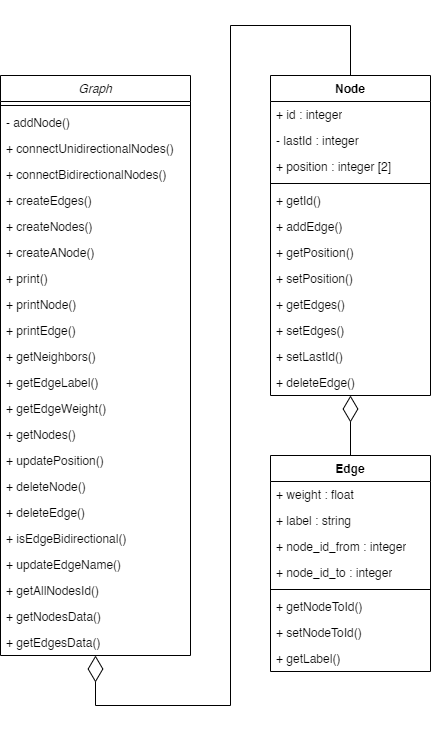
\includegraphics[width=0.7\textwidth]{report/Diagram/classGraph.png}
\caption{Diagramme de class de la class Graph}
\end{figure}

Ainsi, la class graph est composé de la class Node qui est composée de la class Edge

En code, nous l'avons implémenté avec des HashMap:

\begin{lstlisting}[language=java]
HashMap<Integer, Node> nodes;
\end{lstlisting}
\begin{lstlisting}[language=java]
HashMap<Integer, Edge> edges;
\end{lstlisting}

Nous avons choisi les HashMap car elles permettent de directement relier un id de nœud à un lui-même ou bien un id de Nœud à la liaison qu'il a avec un autre sans les numéroter de façon continue. En termes de code, nous n'avons pas à parcourir toute une liste pour trouver l'objet qui nous intéresse, il suffit d'utiliser la ligne suivant :

\begin{lstlisting}[language=java]
Node node = nodes.get(node_to_id);
\end{lstlisting}

\subsection{Recherche d'un itinéraire le plus court entre deux points}

 Pour trouver l'itinéraire le plus court, nous avons utilisé au choix l'algorithme de Dijkstra. \\

Il s'agit d'un algorithme de programmation dynamique. En effet, pour trouver le plus court chemin entre le départ et l'arrivée, on cherche le plus court chemin entre le départ et les nœuds précédents de l'arrivée, puis les nœuds précédents.
Ainsi, l'algorithme de Dijkstra utilise une liste de priorité pour à chaque fois explorer le nœud  avec la valeur la plus faible. Cette structure de donnée est codée ainsi :
\begin{lstlisting}[language=java]
    PriorityQueue<NodeDistance> queue = new PriorityQueue<>();
\end{lstlisting}

Ainsi, pour ajouter un élément ou récupérer l'élément prioritaire, on utilise :
\begin{lstlisting}[language=java]
    queue.add(node)
    node = queue.poll()
\end{lstlisting}

Nous arrêtons la recherche quand le nœud en cours d'exploration est présent dans les nœuds déjà explorés en sens inverse. Pour stocker la liste des nœuds à visiter par ordre de priorité (temps le plus court pour y accéder) nous utilisons la structure du tas qui permet d'accéder rapidement à l'élément ayant la plus petite valeur.


\subsection{Édition et sauvegarde depuis des fichiers}

Le format de fichier choisi est le .txt pour pouvoir éditer un fichier et le charger ensuite, comme demandé en cours. Le fichier a un formatage particulier et les informations sont scindées en 2 : on a d'abord les informations des nœuds, avec le numéro d'identifiant, puis les coordonnées x et y. Ensuite, on a les informations des arêtes, avec l'identifiant du nœud de départ, celui du nœud d'arrivée et le label associé. Ces informations sont délimitées par des drapeaux : "***" pour le début, la limitation entre les 2 types de données et la fin et "*" entre chaque groupe de données (nœud ou arêtes). 

Pour éditer un fichier, on doit commencer par lire ce dernier, ce qui est réalisé avec la fonction "readFile" de la classe Files. Cette fonction lit un fichier texte contenant des informations sur un graphe, extrait ces informations et crée un objet Graph représentant le graphe avec les nœuds et les arêtes correspondants.

Pour lire un fichier, on fait appel à la fonction "writeFile" qui prend un Graph en paramètres, et crée un fichier avec les informations de ce dernier, en respectant le formatage décrit précédemment.


\section{Controler}

\section{Vue}
\subsection{Menu}
\subsection{Draw}

Les fonctions qui permettent de dessiner les différents éléments du Graph sont rassemblées dans la classe Draw. 






\end{document}